
\subsubsection{UC8 - Visualizzazione lista utenti}
\begin{itemize}
	\item \textbf{Attori primari:} utente amministratore;
	\item \textbf{Descrizione:} l'amministratore intende prendere visione della lista degli utenti che hanno accesso al sistema. Per ogni utente vengono visualizzate le seguenti informazioni:
		\begin{itemize}
			\item nome utente;
			\item password.
		\end{itemize}
	\item \textbf{Scenario principale:} l'amministratore visualizza la lista degli utenti;
	\item \textbf{Precondizione:} l'amministratore ha accesso all'elenco degli utenti esistenti;
	\item \textbf{Postcondizione:} l'amministratore ha visionato la lista degli utenti.
\end{itemize}

\subsubsection{UC9 - Creazione utente}
	\begin{figure}[h!]
		\centering
		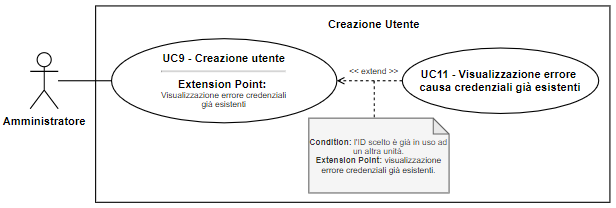
\includegraphics[width=14cm]{images/uc9.png}
		\caption{Diagramma UC9 - Creazione utente}
	\end{figure}
	\begin{itemize}
		\item \textbf{Attori primari:} utente amministratore;
		\item \textbf{Descrizione:} l'amministratore intende aggiungere un nuovo utente, alla lista degli utenti che hanno accesso al sistema;
		\item \textbf{Scenario principale:} l'amministratore crea un nuovo utente, inserendo le rispettive credenziali;
		\item \textbf{Precondizione:} l'amministratore ha accesso all'elenco degli utenti esistenti;
		\item \textbf{Postcondizione:} l'amministratore ha modificato la lista degli utenti creando un utente.
		\item \textbf{Estensione:}
		\begin{itemize}
			\item \textbf{UC11}: l'utente visualizza un messaggio d'errore dovuto al fatto che ha inserito delle credenziali già esistenti.
		\end{itemize}
	\end{itemize}

	\begin{figure}[h!]
		\centering
		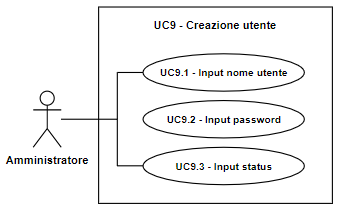
\includegraphics[width=8cm]{images/sottocasi_uc9.png}
		\caption{Diagramma sottocasi UC9 - Creazione utente}
	\end{figure}

\subsubsection{UC9.1 - Input nome utente}
	\begin{itemize}
		\item \textbf{Attori primari:} utente amministratore;
		\item \textbf{Descrizione:} l'amministratore inserisce il nome utente da assegnare all'utente interessato;
		\item \textbf{Scenario principale:} l'amministratore esegue l'input del nome utente;
		\item \textbf{Precondizione:} l'amministratore ha accesso all'elenco degli utenti esistenti;
		\item \textbf{Postcondizione:} l'amministratore ha inserito il nome utente dell'utente interessato.
	\end{itemize}

\subsubsection{UC9.2 - Input password}
	\begin{itemize}
		\item \textbf{Attori primari:} utente amministratore;
		\item \textbf{Descrizione:} l'amministratore inserisce la password da assegnare all'utente interessato;
		\item \textbf{Scenario principale:} l'amministratore esegue l'input della password;
		\item \textbf{Precondizione:} l'amministratore ha accesso all'elenco degli utenti esistenti;
		\item \textbf{Postcondizione:} l'amministratore ha inserito la password dell'utente interessato.
	\end{itemize}

\subsubsection{UC9.3 - Input status}
\begin{itemize}
	\item \textbf{Attori primari:} utente amministratore;
	\item \textbf{Descrizione:} l'amministratore sceglie lo status da assegnare all'utente interessato;
	\item \textbf{Scenario principale:} l'amministratore specifica, tra le opzioni disponibili, lo status da assegnare all'utente;
	\item \textbf{Precondizione:} l'amministratore ha accesso all'elenco degli utenti esistenti;
	\item \textbf{Postcondizione:} l'amministratore ha inserito lo status dell'utente interessato.
\end{itemize}

\subsubsection{UC10 - Rimozione utente}
\begin{itemize}
	\item \textbf{Attori primari:} utente amministratore;
	\item \textbf{Descrizione:} l'amministratore intende eliminare un utente dalla lista degli utenti che hanno accesso al sistema;
	\item \textbf{Scenario principale:} l'amministratore cancella l'utente interessato dalla lista degli utenti;
	\item \textbf{Precondizione:} l'amministratore ha accesso all'elenco degli utenti esistenti;
	\item \textbf{Postcondizione:} l'amministratore ha modificato la lista degli utenti rimuovendo un utente.
\end{itemize}

\subsubsection{UC11 - Visualizzazione errore causa credenziali già esistenti}
	\begin{itemize}
		\item \textbf{Attori primari:} utente amministratore;
		\item \textbf{Descrizione:} l'amministratore visualizza un errore, relativo al fatto che il nome utente che ha tentato di assegnare all'utente è già in uso;
		\item \textbf{Scenario principale:} l'amministratore tenta di inserire un nome utente non valido in quanto assegnato ad un altro utente, ed il sistema risponde con un apposito errore;
		\item \textbf{Precondizione:} l'amministratore ha inserito i dati dell'utente interessato;
		\item \textbf{Postcondizione:} viene visualizzato un errore per informare l'utente che le credenziali utilizzate sono già esistenti.
	\end{itemize}

\subsubsection{UC12 - Visualizzazione mappatura}
	\begin{itemize}
		\item \textbf{Attori primari:} utente amministratore;
		\item \textbf{Descrizione:} l'amministratore prende visione della mappatura dell'ambiente gestito dal sistema;
		\item \textbf{Scenario principale:} l'amministratore visualizza la mappa;
		\item \textbf{Precondizione:} l'amministratore ha accesso alla mappatura dell'ambiente;
		\item \textbf{Postcondizione:} l'amministratore ha visionato la mappatura dell'ambiente.
	\end{itemize}

	\subsubsection{UC13 - Modifica mappatura}
	\begin{figure}[H]
		\centering
		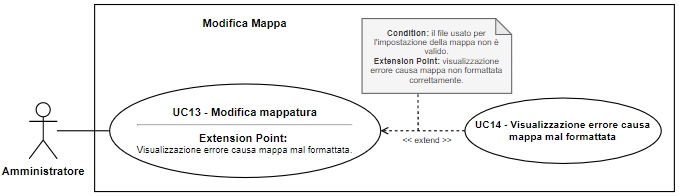
\includegraphics[width=15cm]{images/uc13.png}
		\caption{Diagramma UC13 - Modifica mappatura}
	\end{figure}
	\begin{itemize}
		\item \textbf{Attori primari:} utente amministratore;
		\item \textbf{Descrizione:} l'amministratore applica le modifiche volute alla mappa;
		\item \textbf{Scenario principale:} l'amministratore formatta la mappa nella maniera voluta;		
		\item \textbf{Precondizione:} l'amministratore ha accesso alla mappatura dell'ambiente;
		\item \textbf{Postcondizione:} l'amministratore ha modificato la mappatura dell'ambiente.
		\item \textbf{Estensione:}
		\begin{itemize}
			\item \textbf{UC14:} se si tenta di formattare la mappa erratamente, viene visualizzato un apposito messaggio di errore.
		\end{itemize}
	\end{itemize}

\subsubsection{UC14 - Visualizzazione errore causa formattazione mappa mal formattata}
	\begin{itemize}
		\item \textbf{Attori primari:} utente amministratore;
		\item \textbf{Descrizione:} l'amministratore visualizza un errore, relativo al fatto che la mappa è stata formattata erratamente;
		\item \textbf{Scenario principale:} l'amministratore tenta di formattare erroneamente la mappa;
		\item \textbf{Precondizione:} l'amministratore sta modificando la mappatura dell'ambiente.
		\item \textbf{Postcondizione:} viene visualizzato un errore per informare l'utente che la mappa è stata mal formattata.
	\end{itemize}

\subsubsection{UC15 - Visualizzazione lista unità}
\begin{itemize}
	\item \textbf{Attori primari:} utente amministratore;
	\item \textbf{Descrizione:} l'amministratore intende prendere visione della lista delle unità presenti nel sistema, e per ognuna viene visualizzato il rispettivo ID;
	\item \textbf{Scenario principale:} l'amministratore visualizza la lista delle unità;
	\item \textbf{Precondizione:} l'amministratore ha accesso all'elenco delle unità esistenti;
	\item \textbf{Postcondizione:} l'amministratore ha visionato la lista delle unità.
\end{itemize}

\subsubsection{UC16 - Inserimento unità}
	\begin{itemize}
		\item \textbf{Attori primari:} utente amministratore;
		\item \textbf{Descrizione:} l'amministratore intende aggiungere una nuova unità, alla lista di quelle gestite dal sistema;
		\item \textbf{Scenario principale:} l'amministratore aggiunge l'unità interessata alla lista di quelle già esistenti fornendo il rispettivo ID unità;
		\item \textbf{Precondizione:} l'amministratore ha accesso all'elenco delle unità esistenti;
		\item \textbf{Postcondizione:} l'amministratore ha modificato la lista delle unità inserendo un'unità.
	\end{itemize}

\subsubsection{UC17 - Rimozione unità}
	\begin{itemize}
		\item \textbf{Attori primari:} utente amministratore;
		\item \textbf{Descrizione:} l'amministratore intende eliminare un'unità, dalla lista di quelle gestite dal sistema;
		\item \textbf{Scenario principale:} l'amministratore rimuove l'unità interessata dalla lista di quelle esistenti;
		\item \textbf{Precondizione:} l'amministratore ha accesso all'elenco delle unità esistenti;
		\item \textbf{Postcondizione:} l'amministratore ha modificato la lista delle unità rimuovendo un'unità.
	\end{itemize}